\documentclass{article}
\usepackage[utf8]{inputenc}
\usepackage[T1]{fontenc}
\usepackage{microtype}
\usepackage{newspaper}
\usepackage{sudoku}

\date{\today}
\currentvolume{1}
\currentissue{1}

\SetPaperName{The Daily Hennig}
\SetHeaderName{The Daily Hennig}
\SetPaperLocation{Somerville, MA}
\SetPaperSlogan{``All the News I Feel Like Printing.''}
\SetPaperPrice{Zero Dollars}

\usepackage{graphicx}
\usepackage{multicol}
\usepackage{picinpar}
\usepackage{newspaper-mod} % modifies newspaper style

%%%%%%%%%  Front matter   %%%%%%%%%%

\usepackage{lipsum}
\renewcommand\headline[1]{\begin{center} {\huge \textsl{ #1}}\\ %
			\rule[5pt]{0.8\hsize}{0.5pt}\\ \end{center}}

\begin{document}
\maketitle

\begin{multicols}{3}

\headline{Weather}
% \vspace{-1.5cm}
\center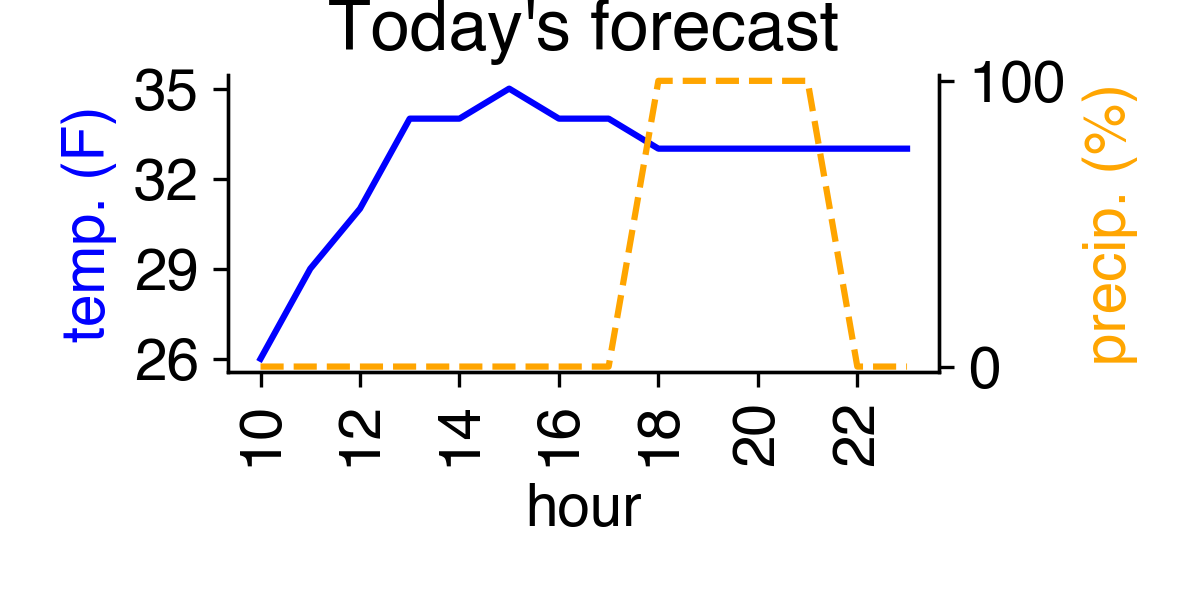
\includegraphics[width=\linewidth]{images/weather-forecast.png}
\noindent\center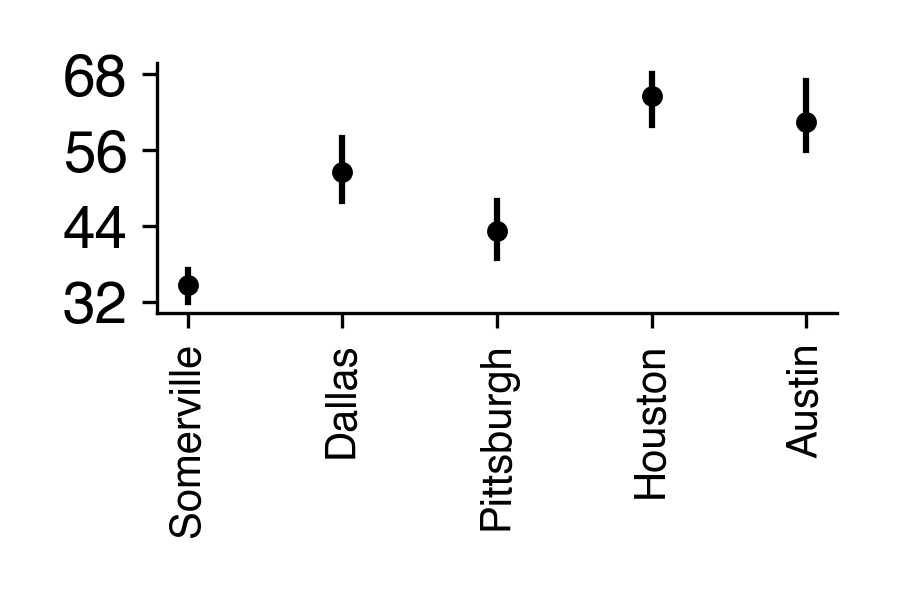
\includegraphics[width=0.75\linewidth]{images/weather-ranges.png}

\headline{Sports}
\begin{center}
\begin{tabular}{|c c c c|}
 \hline
 Col1 & Col2 & Col2 & Col3 \\
 \hline\hline
 1 & 6 & 87837 & 787 \\ 
 \hline
 2 & 7 & 78 & 5415 \\
 \hline
 3 & 545 & 778 & 7507 \\
 \hline
 4 & 545 & 18744 & 7560 \\
 \hline
 5 & 88 & 788 & 6344 \\
 \hline
\end{tabular}
\end{center}

\headline{Comics}
% \vspace{-1.5cm}
\center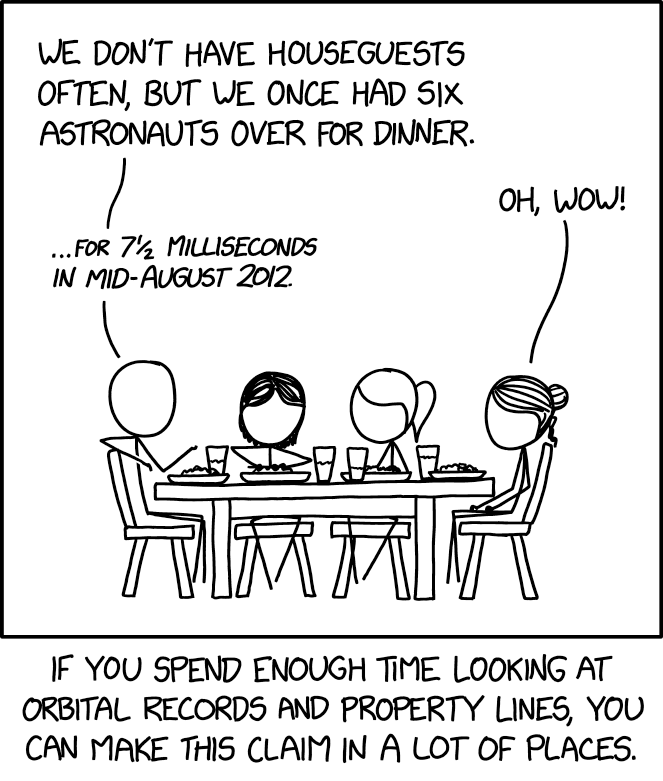
\includegraphics[width=\linewidth]{images/comic.png}

\headline{Games}
\vspace{-0.5cm}
\center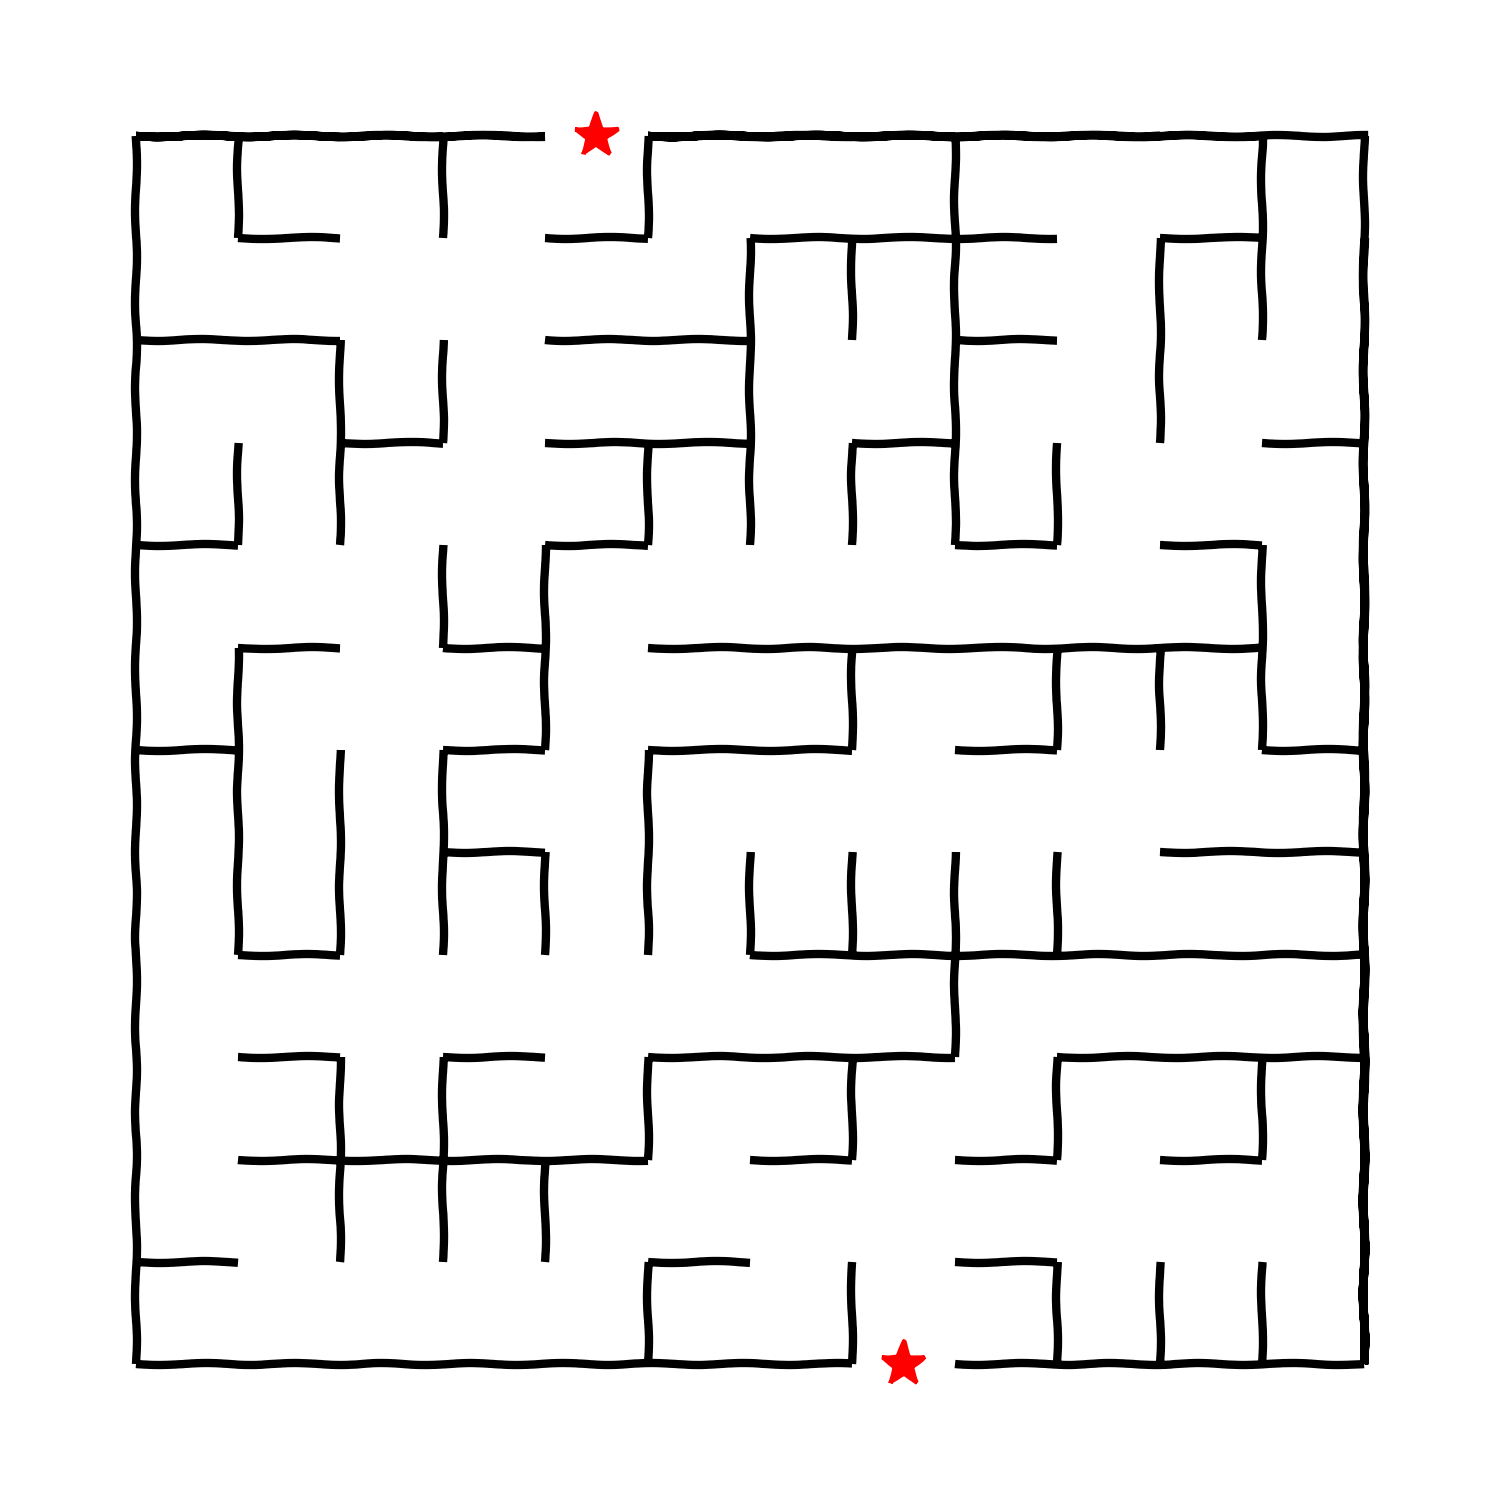
\includegraphics[width=\linewidth]{images/maze_r.png}
\vspace{-0.9cm}
\center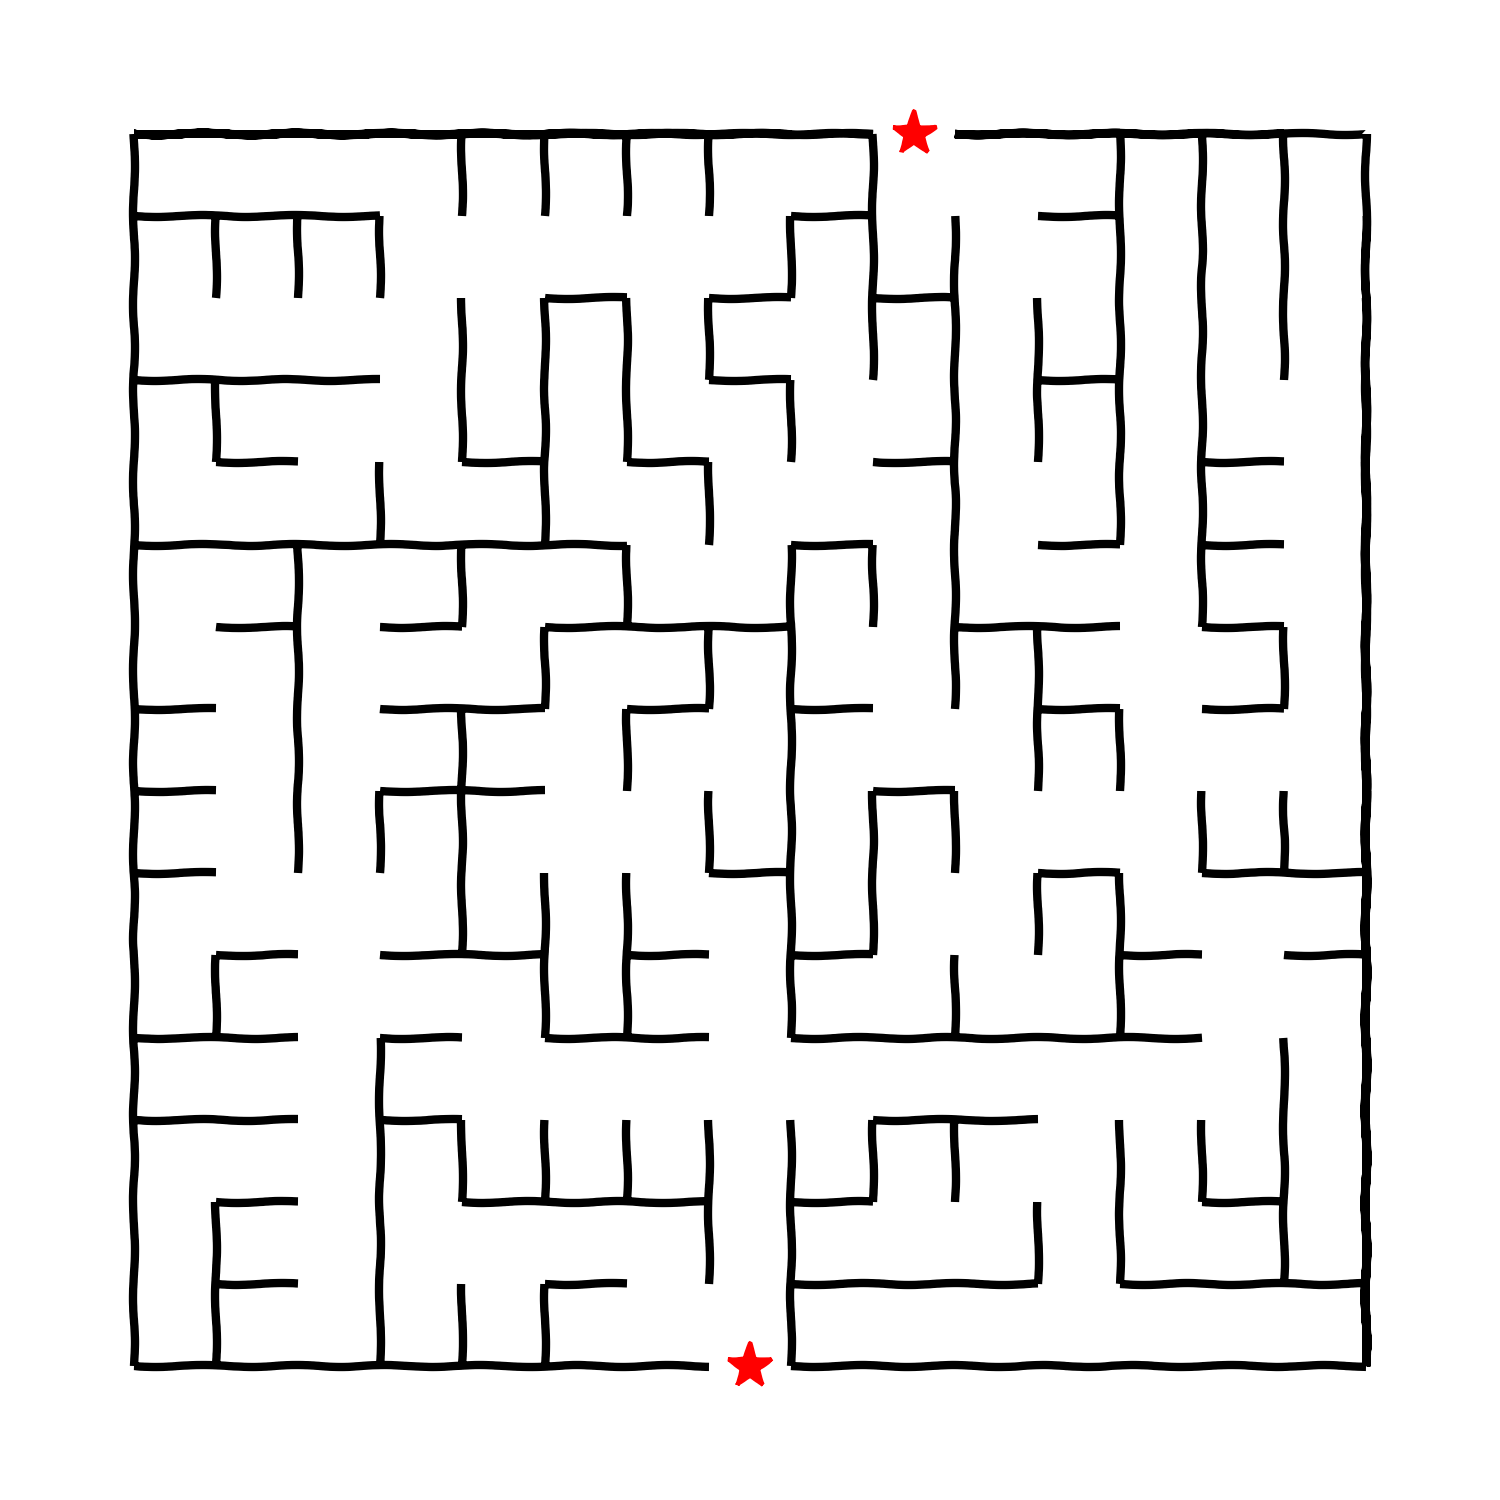
\includegraphics[width=\linewidth]{images/maze_j.png}
\vspace{-0.6cm}

\renewcommand*\sudokuformat[1]{\sffamily#1}
\setlength\sudokusize{4.7cm}
\setlength\sudokuthickline{1pt}
Jess's Sudoku\vspace{0.2cm}
\begin{sudoku-block}
| |2| |4| | |7|9| |.
|6|5|4|7| |9| |3| |.
| |8|7| |2| |4| |5|.
|8|7| |5| |1|6|2|4|.
| |4| |9|7|8| |1| |.
|1| |5|6|4| | | |7|.
| | |2| |6|5|8|7| |.
|5| |3| |9| | |4|1|.
| | |8| | |4|3| |6|.
\end{sudoku-block}

\end{multicols}

\end{document}